\documentclass{beamer}
\usepackage{listings}
\lstset{
%language=C,
frame=single, 
breaklines=true,
columns=fullflexible
}
\usepackage{subcaption}
\usepackage{url}
\usepackage{tikz}
\usepackage{tkz-euclide} % loads  TikZ and tkz-base
%\usetkzobj{all}
\usetikzlibrary{calc,math}
\usepackage{float}
\newcommand\norm[1]{\left\lVert#1\right\rVert}
\renewcommand{\vec}[1]{\mathbf{#1}}
\usepackage[export]{adjustbox}
\usepackage[utf8]{inputenc}
\usepackage{amsmath}
\usetheme{Boadilla}
\providecommand{\pr}[1]{\ensuremath{\Pr\left(#1\right)}}

\title{CSIR UGC JUNE 2013 Q-70}
\author{N.Manaswini-CS20BTECH11035}
\date{}
\begin{document}

\begin{frame}
\titlepage
\end{frame}
\begin{frame}
\frametitle{Question}

\begin{block}{}
Let $X$ and $Y$ be independent random variables each following a uniform distribution on $(0,1)$.Let $W=XI_{\{Y\leq X^2\}}$,where $I_A$ denotes the indicator function of set $A$.Then which of the following statements are true? 

 
\begin{enumerate}
    \item The cumulative distribution function of $W$ is given by
    \begin{align}
     F_W(t)=t^2I_{\{0\leq t \leq 1\}}+ I_{\{t > 1\}}
    \end{align}
    \item $P[W>0]=\frac{1}{3}$ 
    \item The cumulative distribution function of $W$ is continuous
    \item The cumulative distribution function of $W$ is given by
     \begin{align}
        F_W(t)=\frac{2+t^3}{3}I_{\{0\leq t \leq 1\}}+ I_{\{t > 1\}}
     \end{align}
\end{enumerate}
\end{block}

\end{frame}
\begin{frame}
\frametitle{SOLUTION}
Given $X$ is an independent random variable,where $X \in (0,1)$ following a uniform distribution.
\begin{align}
\int_{0}^{1} p_X(x) \mathrm{dx} &=1  \\
\therefore p_X(x)&=1 \label{px}
\end{align}

The PDF for $X$ is
\begin{align}
p_X(x) = 
\begin{cases}
     1 & 0 < x  < 1 \\
     0 & otherwise 
\end{cases}\label{1}
\end{align}
By definition of CDF for $X \in (0,1)$
\begin{align}
F_X(x)&=\int_{0}^{x} p_X(x) \mathrm{dx} \\
      &=x
\end{align}
\end{frame}
\begin{frame}
\frametitle{Solution}
The CDF for $X$ is
\begin{align}
F_{X}(x)  = 
\begin{cases}
      0 & x \leq 0 \\
      x & 0 < x < 1 \\
      1 & otherwise
\end{cases}  \label{2}
\end{align}
\end{frame}
\begin{frame}
\frametitle{Solution}
Given $Y$ is an independent random variable,where $Y \in (0,1)$ following a uniform distribution.\\
\begin{align}
\int_{0}^{1} p_Y(y) \mathrm{dy} &=1  \\
\therefore p_Y(y)&=1 \label{py}
\end{align}
The PDF for $Y$ is
\begin{align}
p_{Y}(y)  = 
\begin{cases}
      1 & 0 < y < 1 \\
      0 & otherwise 
\end{cases} \label{3}
\end{align}
By definition of CDF for $Y \in (0,1)$
\begin{align}
F_Y(y)&=\int_{0}^{y} p_Y(y) \mathrm{dy} \\
      &=y
\end{align}
\end{frame}
\begin{frame}
\frametitle{Solution}
The CDF for $Y$ is
\begin{align}
F_{Y}(y)  = 
\begin{cases}
      0 & y \leq 0 \\
      y & 0 < y < 1 \\
      1 & otherwise 
\end{cases}\label{4}
\end{align}
\end{frame}
\begin{frame}
\begin{block}{Indicator function}
The indicator function of an event $E$ is defined as follows
\begin{align} 
I_{E}(w) =
\begin{cases}
    1 & w \in E \\
    0 & otherwise 
\end{cases} \label{5}
\end{align}
So,indicator function given in question is defined as follows where $X,Y \in (0,1)$ are independent random variables
\begin{align} 
I_{\{Y\leq X^2\}} =
\begin{cases}
    1 & y \leq x^2  \\
    0 & otherwise 
\end{cases} \label{6}
\end{align}
\end{block}
\end{frame}
\begin{frame}
\frametitle{Solution}
$W=XI_{\{X^2 \leq Y\}}$ is defined as follows
\begin{align}
W  = 
\begin{cases}
    x & y \leq x^2 \\
    0 & otherwise
\end{cases}  \label{6}
\end{align}
From above definition
\begin{align}
p_W(W=0) &= \Pr(I_{\{Y\leq X^2\}}=0) \\
         &=\Pr(x^2 <y) \label{7}
\end{align}
\end{frame}
\begin{frame}
\frametitle{Solution}
\begin{block}{$\Pr(x^2<y)$}
This can be found in two ways\\
\begin{enumerate}
\item graphical method
\item convolution
\end{enumerate}
\end{block}
\end{frame}
\begin{frame}
\frametitle{Solution(graphical method)}
\begin{figure}[htb!]
\begin{center}
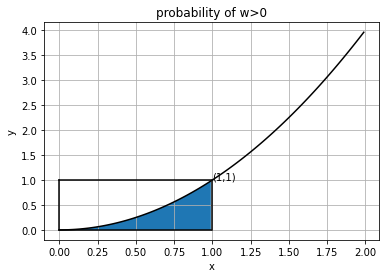
\includegraphics[width=0.4\columnwidth]{assignment8.png}
\end{center}
\end{figure}
From the graph
\begin{align}
\Pr(x^2 \geq y)&= \frac{\mbox{area of shaded part}}{\mbox{Area of rectangle}}\\
               &= \int_{0}^{1} x^2 \mathrm{dx} \\
\therefore P[W>0]&=\frac{1}{3} \\
P[W=0]&=1-\frac{1}{3}=\frac{2}{3} 
\end{align}
\end{frame}
\begin{frame}
\frametitle{Solution(convolution for $\Pr(x^2<y)$)}
Let $Z=X^2-Y$ be a random variable where $Z \in (-1,1)$
\begin{align}
F_{X^2}(u)&= \Pr(X^2 \leq u) \\
          &= \Pr(X \leq \sqrt{u}) \\
          &= F_X(\sqrt{u}) \label{8}
\end{align}
From \eqref{2},The CDF for $X^2$ is
\begin{align}
F_{X^2}(u)  = 
\begin{cases}
      0 & u \leq 0 \\
      \sqrt{u} & 0 < u < 1 \\
      1 & otherwise
\end{cases} \label{9}
\end{align}
\end{frame}
\begin{frame}
\frametitle{Solution(convolution for $\Pr(x^2<y)$)}
By definition of PDF for $X^2 \in (0,1)$
\begin{align}
p_{X^2}(u)&=\frac{\mathrm{d}F_{X^2}(u)}{\mathrm{du}}  \\
          &=\frac{\mathrm{d}\sqrt{u}}{\mathrm{du}} \\
          &=\frac{1}{2\sqrt{u}}
\end{align}
The PDF for $X^2$ is
\begin{align}
p_{X^2}(u)  = 
\begin{cases}
      \frac{1}{2\sqrt{u}} & 0 < u < 1 \\
      0 & otherwise
\end{cases} \label{10}
\end{align}
\end{frame}
\begin{frame}
\frametitle{Solution(convolution  for $\Pr(x^2<y)$)}
\begin{align}
F_{\{-Y\}}(v)&=\Pr(-Y \leq v) \\
          &=\Pr(Y \geq -v) \\
          &=1-F_Y(-v) \label{11}
\end{align}
From \eqref{4},The CDF for $(-Y)$ is
\begin{align}
F_{\{-Y\}}(v)  = 
\begin{cases}
      1-0 & -v \geq 0\\
      1-(-v) & 0 < -v < 1 \\
      1-1 &  -v \leq 1
\end{cases}
\end{align}
Solving this we get
\begin{align}
F_{\{-Y\}}(v)  = 
\begin{cases}
      0 & v \leq -1\\
      1+v & -1 < v < 0 \\
      1 & otherwise 
\end{cases}\label{12}
\end{align}
\end{frame}
\begin{frame}
\frametitle{Solution(convolution  for $\Pr(x^2<y)$)}
By definition of PDF for $(-Y) \in (-1,0)$
\begin{align}
p_{\{-Y\}}(v)&=\frac{\mathrm{d}F_{\{-Y\}}(v)}{\mathrm{dv}}  \\
          &=\frac{\mathrm{d}(1+v)}{\mathrm{dv}} \\
          &=1
\end{align}
The PDF for $(-Y)$ is
\begin{align}
p_{\{-Y\}}(v)  = 
\begin{cases}
      1 & -1 < v < 0 \\
      0 & otherwise
\end{cases} \label{p-y}
\end{align}
\end{frame}
\begin{frame}
\frametitle{Solution(convolution  for $\Pr(x^2<y)$)}
$Z=X^2-Y$ $\implies  z=u+v$\\
\begin{block}{Using convolution}
\begin{align}
p_Z(z)=\int_{- \infty}^{\infty} p_{X^2}(z-v)p_{\{-Y\}}(v) \mathrm{dv} \label{pz}
\end{align}
\end{block}
\begin{align}
-1 &< v < 0 \\
0 < z-v < 1 &\implies z-1 <v <z 
\end{align}
For $z \in (-1,0]$
\begin{align}
p_Z(z)&=\int_{max(-1,z-1)}^{min(0,z)} p_{X^2}(z-v)p_{\{-Y\}}(v) \mathrm{dv}\\
      &= \int_{-1}^{z}\frac{1}{2 \sqrt{z-v}}\mathrm{dv}\\
      &=\sqrt{z+1}
\end{align}
\end{frame}
\begin{frame}
\frametitle{Solution(convolution for $\Pr(x^2<y)$)}
For $z \in (0,1)$
\begin{align}
p_Z(z)&=\int_{max(-1,z-1)}^{min(0,z)} p_{X^2}(z-v)p_{\{-Y\}}(v) \mathrm{dv}\\
      &= \int_{z-1}^{0}\frac{1}{2 \sqrt{z-v}}\mathrm{dv}\\
      &=1-\sqrt{z}
\end{align}
 PDF of $Z$ as follows
\begin{align}
p_{Z}(z)  = 
\begin{cases}
      \sqrt{z+1} & -1 < z \leq 0 \\
      1-\sqrt{z} & 0 < z <1 \\
      0 & otherwise 
\end{cases} \label{13}
\end{align}
\end{frame}
\begin{frame}
\frametitle{Solution(convolution for $\Pr(x^2<y)$)}
By definition of CDF
\begin{align}
F_Z(z)&=\int_{-\infty}^{\infty} p_{Z}(z) \mathrm{dz}\\
\end{align}
for $z \in (-1,0]$
\begin{align}
F_Z(z)&=\int_{-1}^{z} p_{Z}(z) \mathrm{dz}\\
      &=\int_{-1}^{z} \sqrt{z+1} \mathrm{dz}\\
      &= \frac{2}{3}{(z+1)}^\frac{3}{2}
\end{align}
\end{frame}
\begin{frame}
\frametitle{Solution(convolution for $\Pr(x^2<y)$)}
for $z \in (0,1)$
\begin{align}
F_Z(z)&=\int_{0}^{z} p_{Z}(z) \mathrm{dz}\\
      &=\int_{0}^{z} (1-\sqrt{z}) \mathrm{dz}\\
      &= z-\frac{2}{3}{z}^\frac{3}{2}
\end{align}
CDF of $Z$ as follows
\begin{align}
F_{Z}(z)  = 
\begin{cases}
      \frac{2}{3}{(z+1)}^\frac{3}{2} & -1 < z \leq 0 \\
      z-\frac{2}{3}{z}^\frac{3}{2} & 0 < z < 1 \\
      1 & otherwise
\end{cases} \label{14}
\end{align}

\end{frame}
\begin{frame}
\frametitle{Solution}
 using \eqref{14} to find $p_W(W=0)$
\begin{align}
p_W(W=0) &=\Pr(x^2 <y) \\
         &=F_z(0) \\
         &=\frac{2}{3}(0+1)^\frac{3}{2} \\
         &=\frac{2}{3} \label{15}
\end{align}
We need to find PDF of $W$\\
$W=t \implies X=t $ where $t \in (0,1)$
\begin{align}
p_{W}(t) = \int_{- \infty}^{\infty} p_X(t)I_{\{y\leq t^2\}} \mathrm{dy}
\end{align}
\begin{align}
   0 &< y < 1 \label{16} \\
   0 &< y \leq t^2  \label{17}
\end{align}
\end{frame}
\begin{frame}
\frametitle{Solution}
For $ 0 < t < 1 $,
\begin{align}
p_W(t) &= \int_{0}^{min(1,t^2)} p_X(t)I_{\{y \leq t^2\}} \mathrm{dy} \\
       &=\int_{0}^{t^2} p_X(t)I_{\{y \leq t^2\}} \mathrm{dy} \\
       &= t^2 \label{18}
\end{align}

$\therefore$ PDF of $W$ is as follows
\begin{align}
p_{W}(t)  = 
\begin{cases}
  \frac{2}{3}& t=0 \\
  t^2 & 0 < t < 1 \\
  0 & otherwise
\end{cases} \label{19}
\end{align}
By definition of CDF
\begin{align}
F_W(t)&=\int_{-\infty}^{\infty} p_{W}(t) \mathrm{dt}\\
\end{align}

\end{frame}
\begin{frame}
\frametitle{Solution}
for $t \in [0,1]$
\begin{align}
F_W(t)&=\int_{0}^{t} p_{W}(t) \mathrm{dt}\\
      &=\frac{2}{3}+\int_{0}^{t} t^2 \mathrm{dt}\\
      &= \frac{2+t^3}{3}
\end{align}
The CDF  of $W$ is as follows:
\begin{align}
F_W(t)  = 
\begin{cases}
  0 & t<0 \\
  \frac{2+t^3}{3}& 0 \leq t\leq 1\\
  1 & otherwise
\end{cases} \label{20}
\end{align}
\end{frame}
\begin{frame}
\frametitle{Solution}
We need to find $P[W>0]$
\begin{align}
\Pr(W > 0)&= 1- F_W(0) \\
           &=\frac{1}{3} \label{21} \\
\therefore \Pr(W>0)&=\frac{1}{3}
\end{align}
CDF of $W$ is discontinuous at $W=0$.\\
$\therefore$ option $3$ is incorrect.\\
The CDF in \eqref{20} can be written as
\begin{align}
  F_W(t)=\frac{2+t^3}{3}I_{\{0\leq t \leq 1\}}+ I_{\{t > 1\}}
\end{align}
$\therefore$ option $2$ and $4$ are correct.
\end{frame}
\begin{frame}
\frametitle{graphs}
\begin{figure}[htb!]
\begin{center}
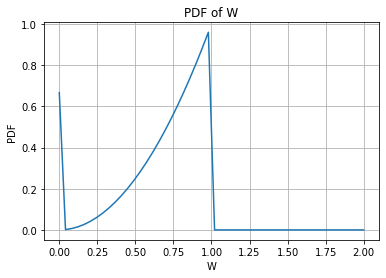
\includegraphics[width=0.4\columnwidth]{assignment8pdf.png}
\end{center}
\end{figure}

\begin{figure}[htb!]
\begin{center}
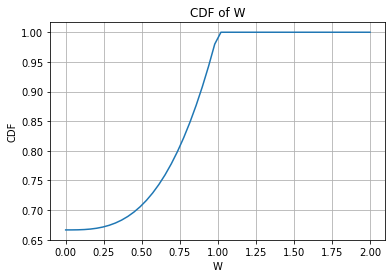
\includegraphics[width=0.4\columnwidth]{assignment8cdf.png}
\end{center}
\end{figure}
\end{frame}
\end{document}
